\chapter[Gaussian tricks]{Hypothesis testing with the CLT} \label{testing} \label{gauss}

This chapter covers most of what we traditionally learn in first-year statistics. 
\comment{
Much of it is obsolete. It covers parameters which we know to have a Normal (aka Gaussian) distribution,
or those things which are derived therefrom. These are nice because the math has already been done, by
people who lived before computers, meaning that we don't need metaphorically heavy machinery to do most of
the calculations here.} Most of the work will consist of taking a dot product, maybe inverting a matrix,
and then looking up a number in a table. 

Everything here depends on the Central Limit Theorem, and more
generally, assumes that your real-world data has a textbook
distribution. Typically, the textbooks state that as the number of draws
$n \to \infty$, the distribution is correct, but whether it is correct
for your data set is a question of \ind{asymptotic theory}.

If your data does not fit the CLT, one option is to work out how your data
is distributed, and then write down a likelihood function. If you are
looking to estimate model parameters, do a maximum likelihood estimation;
if you are looking to test a hypothesis, write down a likelihood ratio
based on the distribution you have just calculated.  Another alternative
is to use the Monte Carlo methods of Chapter \ref{boot} to determine
the properties of your model for $n$ significantly smaller than infinity.

This chapter goes over the process of testing an \airq{oversolved system},
a term defined in detail in Section \ref{mcsec}. The key to constructing
a test is in knowing how the distribution of the data informs the likely
distribution of our estimates of the $\alpha$s, and the key to that
process is the Central Limit Theorem. Section \ref{dist2} will
thus return to probability theory, describing how the CLT affects various
parameter distributions, and then the remainder of the chapter considers
how those parameter distributions can be used to test hypothesized models.

\section{Models and constraints}\label{mcsec}
Before embarking on the process of testing models, it is worth taking
some time to discuss the modeling process and how our models of the
real world translate to estimable parameters.

%A \vocab{hypothesis} is a constraint on otherwise unconstrained parameters. 

Frequently, the statistical and real-world model happen to match very closely.
For example, if we believe that $Y$ is an affine linear sum of $X_1$,
$X_2$, $X_3$, then we are making a claim that 
\begin{equation*}
Y = \alpha_0 + \alpha_1 X_1 + \alpha_2 X_2 + \alpha_3 X_3.
\end{equation*}

In a parallel manner, a statistician could estimate the $\beta$s in the equation
\begin{equation*}
Y = \beta_0 + \beta_1 X_1 + \beta_2 X_2 + \beta_3 X_3 + \epsilon
\end{equation*}
using a standard OLS regression as shown later in this chapter.

Given the parameters estimated using OLS, translating those parameters
to the model is rather trivial:
\begin{align*}
\alpha_0 &= \beta_0\\
\alpha_1 &= \beta_1\\
\alpha_2 &= \beta_2\\
\alpha_3 &= \beta_3.
\end{align*}
However, the translation between parameter estimates and model
parameters easily becomes more complex.  For example, let us say that
we are measuring bicycle usage, $B$, in different  cities.  It would be
a function of the number of motorists $M$, the city's population $P$,
the physical size of the city $S$,  and measures of the availability of
public transportation $T$. But we know that the availability of public
transportation is also a function of the city's population and physical
size. Thus, our model is
\begin{align*}
B &= \alpha_0 M + \alpha_1 P + \alpha_2 \sqrt{S} + \alpha_3 T\\
T &= \alpha_4 P + \alpha_5 \sqrt{S}.
\end{align*}

One option for estimating this model is to run two analogous regressions,
\begin{align*}
B &= \beta_0 M + \beta_1 P + \beta_2 \sqrt{S} + \beta_3 T + \epsilon\\
T &= \beta_4 P + \beta_5 \sqrt{S} + \epsilon.
\end{align*}
Now the correspondence between the two parameters is as trivial as
before ($\alpha_0=\beta_0$, $\alpha_1=\beta_1$, et cetera). This is the
simplest example of \vocab{exactly solved parameters}.
But we get a
distorted view of the effect of city size and population on bicycling
prevalence, because some of those variables' effect is subsumed in the fact that
those factors help to determine whether a city has public
transportation. If the population of a city rises ten percent, ridership
will not rise by $.1 \beta_1$, because $T$ will change as well.

Another option is to substitute $T$ as specified in the second equation into
the first. Then, the model is
\begin{align*}
B &= \alpha_0 M + (\alpha_1 +\alpha_3 \alpha_4) P + (\alpha_2 + \alpha_3 \alpha_5) \sqrt{S}.\\
\end{align*}
The OLS analogue of a linear equation still looks like it did before:
\begin{align*}
B &= \beta_0 M + \beta_1 P + \beta_2 \sqrt{S} + \epsilon.
\end{align*}
Now, the conversion is nontrivial:
\begin{align}
\alpha_0 &= \beta_0     \label{consteq1}\\
\alpha_1 +\alpha_3 \alpha_4 &= \beta_1        \label{consteq2}\\
\alpha_2 + \alpha_3 \alpha_5 &= \beta_2.       \label{consteq3}
\end{align}
Equation \ref{consteq1} still gives us an estimate of $\alpha_0$,
but all our information about  $\alpha_1$ through $\alpha_5$ is
embodied in Equations \ref{consteq2} and \ref{consteq3}. With four
unknowns and two equations, the parameters are \airq{oversolved}. 
\index{undersolved parameter}

We have a better view of the effect of the variable $P$ on $B$, but we
do not have enough information to disaggregate that effect into the
direct effect ($\alpha_1$) and the indirect effect ($\alpha_3 \alpha_4$)
caused by the effect population has on public transport availability
($\alpha_4$). 

Depending on your situation and goals, one setup or the other may be
more appropriate. However, we must acknowledge the limitations of an
undersolved system: $n$ parameter estimates can inform at most $n$ model
parameters.

Now, let us say that a prior study has shown that $\alpha_2= 2.204$.
Discarding the equation for $T$ for now, our model is now:
\begin{align*}
B &= \alpha_0 M + \alpha_1 P + \alpha_2 \sqrt{S} + \alpha_3 T\\
\alpha_2 &= 2.204.
\end{align*}
and after estimating the parameters using a simple OLS estimation, the 
translation from estimated $\beta$s to model $\alpha$s is:
\begin{align*}
\alpha_0 &= \beta_0\\
\alpha_1 &= \beta_1\\
\alpha_2 &= \beta_2\\
\alpha_2 &= 2.204\\
\alpha_3 &= \beta_3.
\end{align*}
Unless we have the incredible luck that $\beta_2=2.20400$, $\alpha_2$ is an
\vocab{oversolved parameter} that has no solution.

There are two things that one can do with an oversolved system. One is
to use the extra constraints to inform the parameter estimation routine;
in the example above, we would estimate the parameters under the
assumption that $\beta_2$ is fixed at 2.204.
You can do this using constrained least squares (Section
\ref{constrainedls}) or via maximum likelihood estimation as in Chapter
\ref{mle}. The other option is to compare the unconstrained version of
the model with the constrained version to see how much distortion occurs
when the constraint binds. This is \airq{testing the constraints}, aka,
a \airq{hypothesis test}.
\index{least squares!constrained}

Recall that the two primary activities of the statistician are estimating
models and testing models.  For an undersolved system, we can neither
estimate nor test the model. For an exactly solved system, we can always
estimate the parameters of the model, but can not verify or refute the
model: you give me a data set, and I will always be able to give you
some set of model parameters. For an oversolved system, we can both
estimate the parameters and test whether the model is correct, because
there will not always be a way to consistently transform the estimated
parameters into model parameters.

Because there is so little persuasive power in an estimated but not
tested model, we often make up
ways to convert an exactly solved system into an oversolved one.
For example, one could add to any equation the additional equation
$\alpha_i = 0$ for all $i$.
By specifying
$Y = \alpha_0 + \alpha_1 X_1 + \alpha_2 X_2 + \cdots$ and $\alpha_1=0$,
we have an oversolved system whose validity we can test. Indeed, this
is the system of equations behind the $t$-tests that are universally
reported with every regression.

This may seem like belaboring the language with such a simple system,
but it is easy to extend this framework to systems of equations, 
exotic constraints, and other variants of the mapping from parameter
estimates to model parameters and testing oversolved equations.

Notably, it could be that the model can't be expressed as an affine
linear sum at all. Perhaps your model is a function in the programming
sense, that takes in a vector of inputs \ci{x1, x2, \dots, xn} and a
vector of parameters \ci{p1, p2, \dots, pm}, runs
through a thousand lines of code, and produces a value \ci{y}. The
problem is still the same---estimate the parameters of the model using
data---but the linear methods are no longer useful. In some cases, there
is a linear system that does not do too much violence to reality; in
other cases, you will need to use the maximum likelihood methods of
Chapter \ref{mle}. However, one could overconstrain the parameters of
this type of model as easily as those above, such as claiming that
\cinline{p1 + p2 == 1}. Chapter \ref{mle} will also discuss likelihood
ratio tests to evaluate the hypotheses embodied in constraints.

By the way, a statement like `We reject
the claim $\alpha_1=0$' is only half right. We are actually rejecting
the claim that both
$Y = \alpha_0 + \alpha_1 X_1 + \alpha_2 X_2 + \cdots$ {\em and}
$\alpha_1=0$. 
The first and second equations are mathematically of equal
status, but the custom is to presume that only the second equation is a
subordinate equation which is under scrutiny. Thus, one would correctly
say `we reject this system of equations'. Having given this caveat, the
remainder of this chapter will use the traditional terminology that
takes the base model as given, reducing
the above pair of equations to the hypothesis $H_0: \alpha_1=0$.

\summary{
\item If the parameters of the model of the real world can not be solved using the 
parameters of the statistical model (e.g., two unknowns and one
equation), then the model is
\vocab{undersolved}. Undersolved variables can neither be estimated nor
tested.
\item If the parameters of the model of the real world can be solved uniquely using the 
parameters of the statistical model, then the model is
\vocab{exactly solved}. Exactly solved variables can be estimated but not
tested.
\item If the parameters of the model of the real world have multiple,
contradictory solutions using the parameters of the statistical model
(e.g., $\alpha_1 = \beta_1$ and $\alpha_1 = 2.2$), then the model is
\vocab{oversolved}. Oversolved systems can be both estimated and
tested.
}


\section{Meet the Gaussian family} \label{dist2}
With the exception of the Normal, the distributions below are distinct
from the distributions of Section \ref{distlist}. The distributions
there
are typically used to describe data that we have observed in the real
world. But having gathered data, we often model the data using techniques
such as linear regressions, that produce means of model parameters,
model variances, and other parameters. Those model parameters have their
own distributions, and those are typically one of the distributions below.

\paragraph{The \ind{Central Limit Theorem}} The CLT is the first piece of magic
that we need.  Assume that we make a series of independent, identically
distributed draws from a fixed underlying population, $x_1, x_2, \dots
x_n$. The underlying population may have {\em any} distribution. Let the
mean of this sequence of draws be $\overline x$. Then as $n\to\infty$,
\comment{
$$\overline X \xrightarrow{a} \left[\mu,{\sigma^2\over n}\right].$$
In fact, we not only have $\overline X$ in the limit, but its distribution:
As $n\to \infty$, }
$$\sqrt{n} \frac{\left(\overline X - \mu\right)}{\sigma} \sim {\cal N}(0,1).$$ 
That is, no matter the underlying population, the mean of a series of
draws will approach a Normal distribution.

With that regularity of nature, we can derive all of the following
distributions.  \label{CLT}

\subsection{Normal\index{Normal distribution}} 

The Normal distribution, defined on page \pageref{normal},
will also be used to describe some of the parameters derived below.
The big problem with the Normal distribution is that it depends on $\sigma$, an
unknown. It also depends on $\mu$, but if the statistic
being tested is unbiased---like most of the estimators of $\beta$ in the
catalog from Chapter \ref{projections}---then you have $\mu$. Thus, much of the trickery in the
section on test design below involves combining distributions in ways
such that the unknown $\sigma$s cancel out.

\subsection{$\chi^2$ distribution}\index{chi squared distribution@$\chi^2$ distribution} 
The square of a Normally-distributed random variable is $\sim \chi^2$
with one degree of freedom, and the sum of $n$ independent
$\chi^2$-distributed variables is also $\sim \chi^2$, with $n$ degrees
of freedom.

\begin{itemize}
\item If $X \sim {\cal N} (0,1)$, then $X^2 \sim \chi^2_1$.

\item If $X_i \sim {\cal N} (0,1)$ for $i=1, \dots, n$, then
$ X_1 + \dots + X_n \sim \chi^2_n$.
\end{itemize}			\label{chisq}

The summation property is immensely useful, because we often have sums
of variables to contend with. The easiest case is the sample variance,
which is a sum of squares. Being a sum of squares of Normally-distributed
elements, it is easy to show that 
\begin{equation}\label{chisqvar}
{\left[\sum_n (x-\overline x)^2\right]\over \sigma^2}\sim \chi^2_{n-1}.
\end{equation}
The numerator there is the sample variance times $n$, so
we can test that the sample variance equals a given $\sigma^2$ with this.

Notice that the sample variance is $\sim
\chi^2_{n-1}$, not $n$, because given the first $n-1$ data points, the
last one can actually be calculated from that data, meaning that we
effectively have the sum of $n-1$ $\{\chi^2_1\}$s plus a no longer
stochastic constant.

\subsection{Student's $t$ distribution\index{t distribution}} Let $\uv$ be
a vector of data (such as the error terms in a regression). Then
${\overline X - \mu \over S/\sqrt{n}}\sim
t_{n-1}$, where $S=\uv'\uv/n$ (a scalar). This is a work of genius by
Mr. Student.\footnote{\airq{Student} is actually Mr. William Sealy
Gosset, who published the t test in 1908 based on his work as an employee
of the Guinness Brewery. \index{Student} \index{William S Gosset}}
By dividing a normal by $\sqrt{\chi^2_{n-1}\over (n-1)}$, the unknown
$\sigma$s cancel, and we have a function whose elements are all known,
and its distribution.  If $n=2$, we call it a \ind{Cauchy distribution}.
\label{tstat}


\subsection{$F$ distribution\index{F distribution}}  This is the same cancel-the-$\sigma$s trick as with the $t$, but here the form
is $[\chi^2_m/m]/[\chi^2_n/n]\sim F(m,n)$. For example, if the numerator
is a ${\cal N}(0,1)$, and the denominator is a $\chi^2$ based on the
sample variance, then this is the square of the $t$ statistic.
The $\chi^2$ distribution 
allows simple one-tailed hypothesis tests, but if you want to test a
multivalued hypothesis, then you need to do an $F$ test.

\subsection{Lookup tables}
There are three things that cover most of what you will be doing with a
distribution: finding values of its PDF, values of its CDF, and inverse
values of its CDF.
Here are the functions to look up the value of the PDF at a given point:

\begin{lstlisting}
double gsl_ran_gaussian_pdf (double X, double SIGMA);
double gsl_ran_tdist_pdf (double X, double df);
double gsl_ran_fdist_pdf (double X, double df1, double df2);
double gsl_ran_chisq_pdf (double X, double df);
\end{lstlisting}

The prefix \ci{gsl\_ran} indicates that these
functions are from the random number generation module
(\ci{gsl/gsl\_randist.h}). Random number generation itself will be
delayed to page \pageref{randomnumbers}. Notice that there is no mean
for the Normal, so we may need to modify $X$ accordingly, e.g., if $X$
is drawn from a ${\cal N}(7,1)$, then you will need to ask the GSL for 
\ci{gsl\_ran\_gaussian\_pdf(X-7, 1)}.


The next distribution calculation found in tables in the back of
statistics texts is calculating the CDF above or below a point. 
The \cinline{P-}functions below calculate the CDF below a point, i.e.
$\int_{-\infty}^X f(y) dy,$
while the \cinline{Q-}functions calculate the CDF above a point, i.e.
$\int^{\infty}_X f(y) dy.$
These will obviously add to one, so you can express any area in terms of whichever function is clearest.

For example, if we find that our Normally distributed mean is 2.2 standard
deviations above zero, then we can reject the one-tailed hypothesis that
the mean is less than or equal to zero with probability \cinline{1 - gsl\_cdf\_gaussian\_Q(2.2, 1) ==
gsl\_cdf\_gaussian\_P(2.2, 1)}.

Here is the list of functions:
\index{Gaussian distribution|see{Normal distribution}}
\index{chi squared distribution@$\chi^2$ distribution!gsl\_cdf\_chisq\_P@\cinline{gsl\_cdf\_chisq\_P}}
\index{t distribution!gsl\_cdf\_tdist\_P@\cinline{gsl\_cdf\_tdist\_P}}
\index{F distribution!gsl\_cdf\_fdist\_P@\cinline{gsl\_cdf\_fdist\_P}}
\index{Normal distribution!gsl\_cdf\_gaussian\_P@\cinline{gsl\_cdf\_gaussian\_P}}
\ttindex{gsl\_cdf\_...}
\begin{lstlisting}
double gsl_cdf_gaussian_P (double X, double SIGMA);
double gsl_cdf_tdist_P (double X, double NU);
double gsl_cdf_fdist_P (double X, double NU1, double NU2);
double gsl_cdf_chisq_P (double X, double NU);
\end{lstlisting}
\dots plus all of these with the \cinline{P} replaced by a \cinline{Q}.


In the other direction, we may want to know where we will need to be to reject a hypothesis with 95\%
certainty. For example, a value-at-risk oriented regulator will want to know what a bank is likely to lose 
one day in the month. That is, what is the value of the 1-in-20, or 5\%, point on the CDF?
Assuming a Normal(M,S) distribution of profit and loss,\footnote{This assumption is false. Securities
typically have \ind{leptokurtic} (fat-tailed) returns; see page \pageref{kurt1}.} the bank will report a \ind{value at risk} of {\tt
gsl\_cdf\_gaussian\_Pinv (0.05, S)+M}. Here are the requisite function declarations:
\index{chi squared distribution@$\chi^2$ distribution!gsl\_cdf\_chisq\_Pinv@\cinline{gsl\_cdf\_chisq\_Pinv}}
\index{t distribution!gsl\_cdf\_tdist\_Pinv@\cinline{gsl\_cdf\_tdist\_Pinv}}
\begin{lstlisting}
double gsl_cdf_gaussian_Pinv (double P, double SIGMA);
double gsl_cdf_chisq_Pinv (double P, double NU);
double gsl_cdf_fdist_Pinv (double P, double NU1, double NU2);
double gsl_cdf_tdist_Pinv (double P, double NU);
\end{lstlisting}
\dots plus all of these with the \cinline{P}s replaced by \cinline{Q}s.
The inverse for the CDFs of the F distribution is a new addition as of
April 2006 (GSL version 1.8), and so may not yet be available on prepackaged
distributions of the GSL.


\summary{
\item The Central Limit Theorem applies to the parameters
of almost all statistical models---that is, the parameters' distribution approaches a Normal
distribution as the number of observations $n \to \infty$.
\item The square of a Normal distribution is a $\chi^2$ distribution.
\item Both of these distributions rely on a variance $\sigma$ which is
unknown. We can guess at $\sigma$, but then our confidence intervals are
mere approximations as well.
\item The ratio of a Normal over the square root of a transformed $\chi^2$ distribution 
is a $t$ distribution. In the transformation, the unknown $\sigma$s
cancel out, so a valid confidence region can be constructed.
\item The ratio of two $\chi^2$ distributions is an $F$ distribution.
Again, the unknown $\sigma$s cancel out.
}



\section{Testing a hypothesis}




We have all the ingredients we need to test a hypothesis; all that
remains is to glue them all together. For example, in the last chapter, the code
found the coefficient vector \cinline{beta} and \cinline{xpx\_inv}, which is the
variance-covariance matrix of \cinline{beta}.  Assume for now that \cinline{beta}
is Normally distributed (for example, the original data set consists
of iid draws from a homoskedatic distribution). Then we can use the
above functions to find the probability that each element of \cinline{beta}
is different from zero:

\lstset{texcl=true} \label{normalassumption} 
\begin{lstlisting}
//We enter with the vector $\betav$ and matrix {\tt xpx\_inv}
int i;
double confidence[beta->size];
for (i=0;i< beta->size; i++){
    double mean = fabs(gsl_vector_get(beta,i));
    double stddev = sqrt(gsl_matrix_get(xpx_inv, i,i));
    confidence[i] = gsl_cdf_gaussian_Q(mean, stddev);
    confidence[i] -= .5;
    confidence[i] *= 2;
}
\end{lstlisting}
\lstset{texcl=false}
\exercise{
The last two steps to the code above are the poor man's way to convert from the one-tailed area below \cinline{beta}
to a two-tailed area between $\pm$\cinline{beta}. If \ci{confidence[i] <
0.5}, then it will output a negative number.

Write a function with header \ci{double two\_tailify(double
*one\_tail)}, that takes in a one-tailed confidence level and returns a
two-tailed confidence level, assuming a symmetric distribution. 

This is infrequently done, but what would be the correct means of
calculating a two-tailed interval for an asymmetric distribution?
}


\subsection{The t-test} \label{ttest} \index{t test|(textbf}
\index{t test!apop\_t\_test@\cinline{apop\_t\_test}}
\index{t test!apop\_paired\_t\_test@\cinline{apop\_paired\_t\_test}}
Among the most common and simplest questions one asks is: are two 
sets of observations from the same process? Chapter \ref{sql} already showed how one
would do such a test; let us briefly revisit the process now.
Let \cinline{n\_side} be the income of households
drawn from the side of town North of the railroad tracks, and
\cinline{s\_side} be the income of households drawn from the South side of
town. Are North side incomes different from South side incomes? 

If $\mu$,
$\sigma^2$, and $n$ are the estimated mean, variance, and actual count
of elements of each data set,
$${\mu_a + \mu_b \over \sqrt{\sigma^2_a/n_a + \sigma^2_b/n_b}} \sim t_{n_a + n_b -2}.$$
Using the ingredients above, the reader could construct a function to
test the hypothesis that the number above, the $t$-statistic, is
different from zero for any given confidence level. Apophenia provides a
high-level function to do the work for you:

\cindex{apop\_t\_test}
\begin{lstlisting}
gsl_vector *a = gather_data("n_side");
gsl_vector *b = gather_data("s_side");
apop_data  *t = apop_t_test(a, b);
apop_data_show(t);
\end{lstlisting}
As per the discussion on page \pageref{testoutput}, Apophenia's testing
functions return a data table listing test statistics, degrees of
freedom, confidence, et cetera. You can print the entire set as above or
just pull a single element, e.g.,
\cindex{apop\_data\_get\_tn}
\begin{lstlisting}
double pval = apop_data_get_tn(t, "p_val%", -1);
\end{lstlisting}

Now let us say that the data is paired, in the sense that for each
element in the first set, there is an element in the second set that is
related; put another way, this means that for each element $a_i$, there
is a corresponding element $b_i$ such that the difference $a_i - b_i$
makes real-world sense. For example, we could look at student scores on
a test before a set of lessons and the same students after the lessons.
Then, rather than looking at the $t$-distribution for the before data
and comparing it to the $t$-distribution for the after data, we could
look at the vector of differences $a_i - b_i$ and test where zero falls
in the appropriate $t$-distribution. This is generally a more powerful test,
meaning that we are more likely to reject the null hypothesis of no
difference between the two vectors, therefore the paired $t$-test is
generally preferable over the unpaired version above (when it is
applicable). Apophenia provides the \cind{apop\_paired\_t\_test}
function to run this test where appropriate.

\paragraph{Regression parameters} Above, the $t$ test was used on sample
data, but it is also typically applied to regression parameters.
Traditionally, the test claims that $\beta_i=0$ for each $i$. This is
such a common test that \ci{apop\_OLS.estimate}\cindex{apop\_OLS} runs
the test automatically, storing the result in
\ci{output\_estimate->par\-a\-met\-ers->ma\-trix}.

\exercise{How would you modify the code on page
\pageref{normalassumption} to accommodate the fact that
OLS parameters are $t$-distributed?}


 \index{t test|)textbf}

\subsection{The $\chi^2$ test}
\index{chi squared test@$\chi^2$ test}
One quick application of the $\chi^2$ distribution is for testing
whether a variance takes on a certain value. We posit that the
denominator of Equation \ref{chisqvar} is a fixed number, and then check
the $\chi^2$ tables for the given degrees of freedom.

The summation property makes it easy for us to sum together individual
tests to form more elaborate tests. 

To give one common example, say that we have a two-by-two array of
events:

\renewcommand\arraystretch{1.1}
\begin{center}
\begin{tabular}{lccc}
    & Left  & Right & $\Sigma$\\
\hhline{~--~}
\multicolumn{1}{c|}{Up}& 30    & 86    & \multicolumn{1}{|c}{116}     \\
\multicolumn{1}{c|}{Down}& 24    & 38  & \multicolumn{1}{|c}{62}     \\
\hhline{~--~}
$\Sigma$& 54    & 124    & 178
\end{tabular}
\end{center}

Is the incidence of Up/Down correlated to the incidence of Left/Right,
or are the two independent? \citet{pearson:chisq} notes that
if Up/Down were a Bernoulli draw with probabilities $p_U$ and $p_D$, and Down/Left
were a separate, independent Bernoulli draw with probabilities $p_R$ and
$p_L$, then the expected value of 
Up/Left would be $E_{UL}=np_Up_L$, the observed variance
would be equal to $E_{UL}$, and notating the actual incidence of Up/Left
as $O_{UL}=30$, the observed variance over the actual variance 
$(O_{UL} - E_{UL})^2/E_{UL} \sim \chi^2$. Similarly for the other three cells,
so the sum 
\begin{equation}
{(O_{UL} - E_{UL})^2\over E_{UL}} +
{(O_{UR} - E_{UR})^2\over E_{UR}} +
{(O_{DL} - E_{DL})^2\over E_{DL}} +
{(O_{DR} - E_{DR})^2\over E_{DR}} 
\sim \chi^2.\label{chisqeqn}
\end{equation}

Figure \ref{fisher} shows how one would calculate this. The first
function, \ci{find\_marginals}, calculates $p_U$, $p_L$, and their
complements. The \ci{calc\_chi\_squared} function calculates Equation
\ref{chisqeqn}. Notice how the \ci{one\_chi\_sq} function, combined with
a text editor's cut and paste facility, makes writing \ci{calc\_chi\_squared} very easy.
Finally, \ci{main} gathers the data and calls the above functions.

The distribution of means of a series of Binomial draws will approach a Normal 
as $n\to \infty$, but for many situations, $n$ is closer to around ten.
For such a case, \citet{fisher:exact} calculated the probability of a
given table using direct combinatorial computation. The equations for
the \ind{Fisher exact test} are a mess, but the story is the same
as above---its null hypothesis is that Up/Down and Left/Right
are independent---and its calculation is trivial: just call
\cind{apop\_test\_fisher\_exact}, as in Figure \ref{fisher}.

\codefig{fisher}{The Fisher exact test.}



\subsection{The $F$ test\index{F test}}\label{ftestsec}
We can use the $\chi^2$ distribution to test two-tailed
tests ($a \neq b$) because of all the squaring involved. To test a
one-tailed test ($a > b$), we could use the $t$ test for one variable,
or an $F$ test for a combination of multiple variables.

Say that $H_0$ asks, is ${\Qv'
\betav} = \cv$?  This is a very versatile question. E.g., $\Qv =
\vector{1\cr 0\cr 0}$ plus $\cv = [7]$ gives $H_0: \beta_1 = 7$. Or, $\Qv = \vector{1 \cr
-1}$ and $\cv = \vector{0}$ gives $H_0: \beta_1=\beta_2$. 
Or, say we want to test that $\beta_2 = 2\beta_3$. Then let $\Qv=\vector{0 \cr 1 \cr -2}$ and $\cv = 0$.
To test multiple hypotheses at once, simply stack the above:
\begin{equation}
\begin{matrix}\Qv' = \vector{1 & 0 & 0  \cr
                0 &1 &-2} 
                & \cv = \vector{7 \cr 0}\end{matrix}.\label{qc}\end{equation}

I dare
say that every linear hypothesis having to do with a mean or a $\beta$ can be
fit into this form.\footnote{If our concern is a mean, then set
$\yv=$your data, $\xv=$ a column of ones, and $\beta$ will then be
$\mu$. Recall that we typically expect that the first column of our data
set $\Xv$ to
be a column of ones anyway.}
Define $q$ to be the number of constraints (columns
of $\Qv$), $N$ the sample size, and $K$ the number of parameters to be
estimated ($\betav$).

Let $\Xuv$ represent $\Xv$ normalized so that each column has mean
zero.\footnote{That is, \cinline{X\_underbar =
apop\_matrix\_normalize(X, 'c', 'm')}.\cindex{apop\_matrix\_normalize}}
Now, if $H_0$ is true and we are using OLS, then $\Qv' \betav \sim {\cal
N}(\cv, \sigma^2 \Qv' (\Xuv'\Xuv)^{-1} \Qv)$,\footnote{For any other
method, the form of the variance is $\Qv'$(the variance from section
\ref{cat})$\Qv$.} and we now have a linear combination of the square of
standard Normals. The $\chi^2$ statistic is:

\begin{equation}		\label{chi1}
{(\Qv'\hat\betav - \cv)' [\Qv' (\Xuv'\Xuv)^{-1} \Qv]^{-1} (\Qv' \hat\betav - \cv)
\over \sigma^2} \sim \chi^2_q
\end{equation}

If we are testing a variance, we'd have 

\begin{equation}		\label{chi2}
{{\bf u}' {\bf u} \over \sigma^2} \sim \chi^2_{N-K}
\end{equation}



As above, we can divide Equation \ref{chi1} by Equation \ref{chi2}
to give us a statistic with an $F$ distribution and no unknown
$\sigma^2$ element:


\wideeqnbox{(\textwidth - \mwidth)}{
%\begin{equation}	
{N-K\over q}
{(\Qv'\hat\betav - \cv)' [\Qv' (\Xuv'\Xuv)^{-1} \Qv]^{-1} (\Qv' \hat\betav - \cv)
\over \uv' \uv } \sim F_{q,N-K}. \label{ftest}
%\end{equation}	
}

If you have read this far, you know how to code all of the operations
in Equation \ref{ftest}.  But fortunately, 
Apophenia includes a function that will calculate Equation \ref{ftest}
for you.
\index{F test!apop\_F\_test@\cinline{apop\_F\_test}}
To do this, you will need to feed the function a $\betav$ vector, and a
matrix $\Qv'$ plus a vector $\cv$ that indicate the set of hypotheses
you wish to test. Notice that each {\em row} of the input matrix represents a
hypothesis. Also, recall that functions ending in \cinline{calloc} allocate
a matrix or vector and simultaneously set every element to zero, giving
you a blank slate to fill. Thus, if you already have a data set, and
would like to run an OLS regression and then test the joint hypothesis
of Equation \ref{qc}, here's what you'd type:
\begin{lstlisting}
apop_estimate *e = apop_OLS.estimate(data, NULL);
gsl_matrix *Q   = gsl_matrix_calloc(3,2);
gsl_vector *c   = gsl_vector_calloc(2);
gsl_matrix_set(Q, 0, 0, 1);
gsl_matrix_set(Q, 1, 1, 1);
gsl_matrix_set(Q, 1, 2, -2);
gsl_vector_set(Q, 0, 7);
apop_data *f = apop_F_test(e, Q, c);
apop_data_show(f);
\end{lstlisting}

        \eject
Here is a useful simplification.
Let $R^2$ be the coefficient of determination (defined further below),
$n$ be the number of data points, $K$ be the number of parameters
(including the parameter for the constant term), and $\phi$ be the
$F$-statistic
based on $\Qv = {\bf I}$ and $\cv = {\bf 0}$. Then it can be shown that 
\begin{equation}
\frac{(n-K) R^2}{K (1-R^2)} = \phi.    \label{rsqandf}
\end{equation}
Since statistical custom is based on the availability of computational
shortcuts, this specific $F$-test often appears in the default output
of many regression packages.  \index{R squared@$R^2$}

\exercise{\label{randfexercise} \index{SSE} \index{SSR}
Verify the identity of Equation \ref{rsqandf} using Equation
\ref{ftest} and these definitions:
\begin{align*}
R^2 &\equiv \frac{SSR}{SSE},  
\intertext{where}
    SSR &\equiv \sum{(y_{\rm est}-\overline y)^2},
\intertext{$\yv_{\rm est}\equiv \Xv\betav$ (the estimated value of $\yv$), and}
    SSE &\equiv {\uv'\uv}.
    %&= \frac{\sum{(y-\overline y)^2}}{\uv'\uv}.
\end{align*}
}

It is up to you
to decide whether the test statistic in Equation \ref{rsqandf} is
relevant for the situation you are dealing with, but because it
is a custom to report it, Apophenia facilitates this hypothesis
test by assuming it as the default when you send in {\tt NULL}
variables, as in \cinline{apop\_F\_test(estimate, NULL, NULL)}. That is,
if $\Qv'=$\cinline{NULL}, Apophenia assumes ${\bf Q}=={\bf I}$ and if
$\cv=$\cinline{NULL}, Apophenia assumes ${\bf c} == {\bf 0}$.

\exercise{Verify the identity of Equation \ref{rsqandf} by running a
linear regression on your favorite data set, and then passing the
\cinline{apop\_estimate} thus produced to \cind{apop\_F\_test} to find
the $F$ statistic and \cind{apop\_coefficient\_of\_determination} to
find the SSE and SSR.}


\summary{
\item The simplest hypothesis test regarding the parameters of a model
is the $t$ test. It claims that the mean of a data set is different from
a given value of $\mu$. A special case is the claim that the mean of two
data sets differ.
\item The $\chi^2$ test is the next step of complication, allowing the
comparison of linear combinations of allegedly Normal parameters. But
since everything is squared to get the $\chi^2$ parameter, it can not
test asymmetric one-tailed hypotheses.
\item The $F$ test provides full generality, and can test both
one-tailed and two-tailed hypotheses.
}


\comment{
\subsection{The F-test}
But we have the whole variance-covariance matrix to work with, not just
the diagonal, so we can readily test any joint hypothesis that suits
our fancy. First, we need a means of expressing the hypothesis.
}

\comment{
\section{Good ol' OLS}
This section would discuss how to write your very own \cinline{regress}
function, which, as noted above, just consists of solving for the $\beta$
in $(X'X)\beta = X'Y$.  The last chapter showed us the code to find the
betas with the smallest squared error; this section will cover testing
hypotheses about those betas.

\subsection{GLS} Generalized least squares refers to any method that
uses a variance-covariance matrix that isn't the identity matrix. Having
written our \cinline{regress} function, it's almost trivial to generalize
to GLS. But the fun of GSL is in working out what that matrix should be.
This section would give examples of favorites such as AR-1 processes
from time series analysis (and hey, why not AR-$N$?).

The easiest thing to do is simply calculate the variances and covariances of the data itself:

%\begin{verbatim}
\begin{lstlisting}
#include "gsl_convenience_fns.h"
gsl_vector_view one_col, another_col;
gsl_matrix *var_covar=gsl_matrix_alloc(data->size2, data->size2);
int i,j;

for(i=0;i< data->size2; i++){
   for(j=0;j<= i; j++){
      one_col = gsl_matrix_column(data, i);
      another_col = gsl_matrix_column(data, j);
      covar = cov(&one_col.vector, &another_col.vector);
      gsl_matrix_set(var_covar, i, j, covar);
      if (j!=i) gsl_matrix_set(var_covar, j, i, covar);
   }
}
\end{lstlisting}
%\end{verbatim}

Now that we've got this variance-covariance matrix, $\Sigma$, we can
apply the formula $\beta_{GLS} = (X'\Sigma X)^{-1} (X'\Sigma Y)$.
}

\comment{
This gives us  $N\cdot (N+1)/2$ covariances that need to be calculated; your data is probably not up to
the task of providing enough information to allow this to be estimated, in which case you will need to
compromise and impose some number of restrictions. 

For example, FGLS (Feasible GLS) assumes that the var-covar matrix is of the form 
$$\left[\matrix{
1 &\rho & \rho^2 & \rho^3\cr
\rho &1 & \rho  & \rho^2\cr
\rho^2 & \rho & 1 & \rho\cr
\rho^3 & \rho^2  & \rho &1\cr
}\right].$$
This makes life easy because we now only have one variable to estimate.
}

\section{\ind{ANOVA}} ANOVA is a contraction for \vocab{analysis
of variance}, and is a catch-all term for a variety of methods that
aim to decompose a data set's variance into subcategories. Given a few
variables and a few groups, is there more variation between groups or
within groups? Can the variation in a dependent variable be attributed
primarily to some independent variables more than others?

\paragraph{Producing the data set} The typical ANOVA data set is a grid
where each row is a subject or group, and each column is a treatment or
experiment; not all cells need to be filled. In the context of the
database discussion, it is a \vocab{crosstab}, which differs slightly
from the usual data sets.

This section forthcoming.

\section{Goodness of fit}
\index{goodness of fit}

Errors have to be normally distributed, or else
the whole OLS system here does not apply. Many stats package user's manuals
suggest plotting the errors and then squinting at the picture; you can
do this using \cinline{apop\_plot\_histogram}. 
A slightly more rigorous alternative means of testing for Normality
is to check the higher moments of the Normal distribution
\citep{bowman:shenton}.  This is the
traditional test, because it is computationally simple; below, a more
general chi-squared goodness-of-fit test is presented.

A Normal distribution has only two parameters, the mean and the
standard deviation, and everything else about the Normal distribution is
defined therefrom. Notably, the third moment is zero, and the fourth
moment is $3 \sigma^4$. 
Un-normalized kurtosis $>3$ is known as \vocab{leptokurtic} and $<3$ is
known as \vocab{platykurtic}; see Figure \ref{tailfig} for a mnemonic.

\begin{figure*}[tb]
%\hspace{-.3in}\scalebox{0.7}{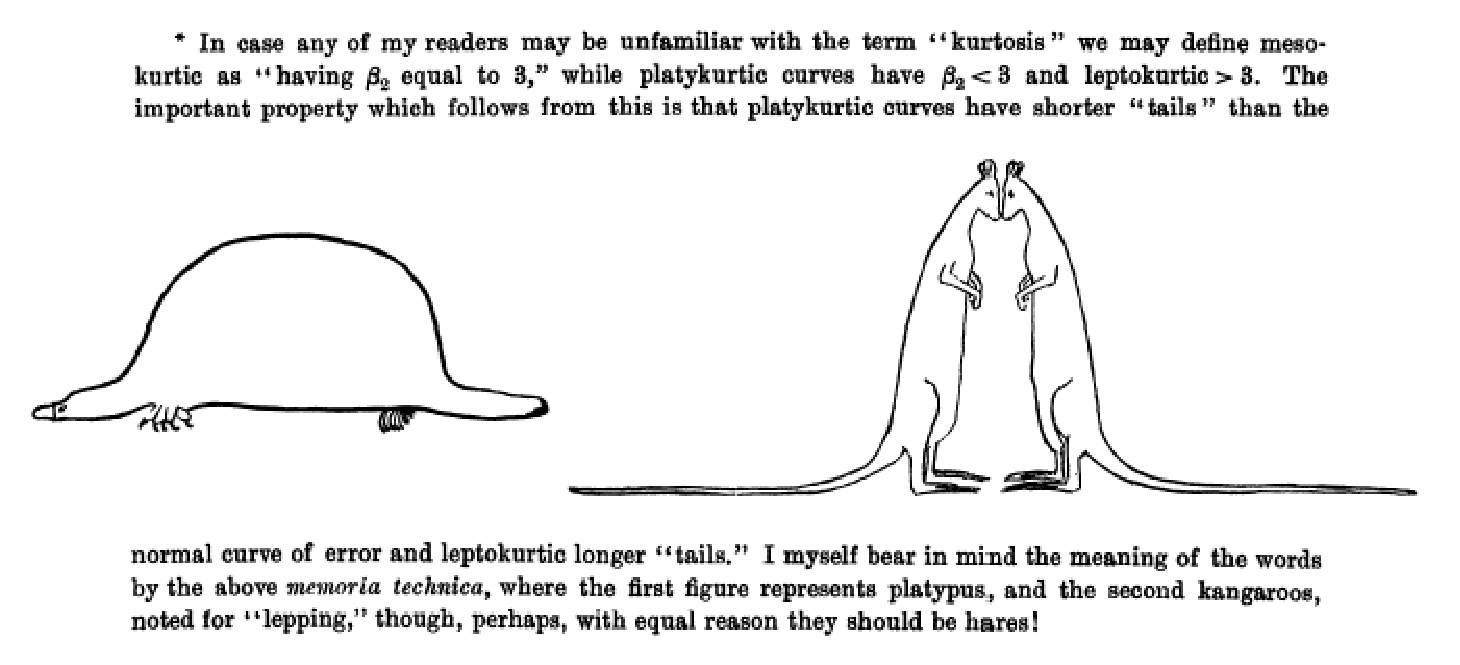
\includegraphics{kurtosis.eps}}
\hspace{-.3in}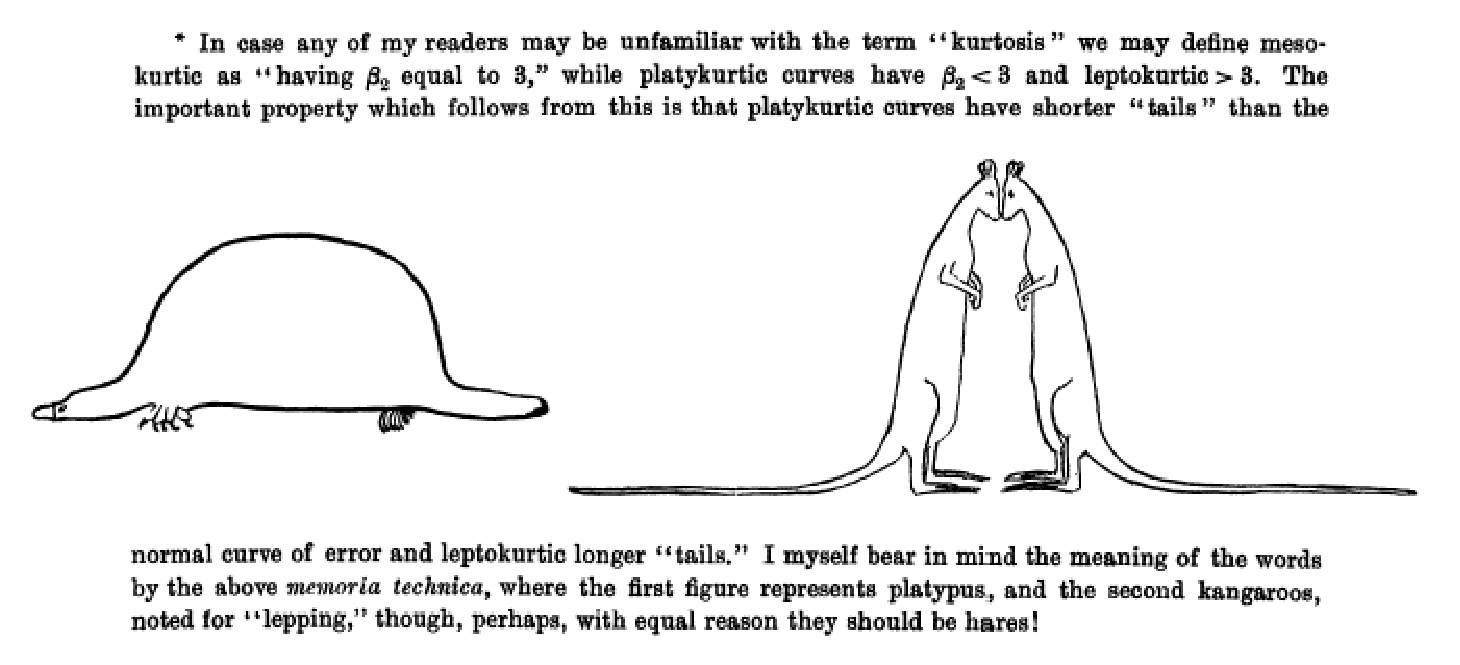
\includegraphics[width=\textwidth*\real{1.1}]{kurtosis.eps}
\caption{Leptokurtic, \ind{mesokurtic} and \ind{platykurtic}, illustration by Gosset in {\em Biometrika} \citep[p 160]{student:errors}.\index{Student} \index{William S Gosset}\index{leptokurtic}}
\label{tailfig}
\end{figure*}

\marginalia{13}{Kurtosis minus three}{
There is some debate as to whether the kurtosis of a ${\cal N}(0,1)\equiv 3$
or $\equiv 0$. This is simply a definitional issue: some prefer to
normalize all reported kurtoses by subtracting three from the actual
fourth moment. For example, the GSL does the normalization; Apophenia does not.
Bear this in mind when interpreting kurtosis output. If you see a
negative kurtosis, then you are guaranteed that you are getting
normalized kurtosis, since a fourth power can never be negative.
\index{kurtosis}}

We have already written everything we need to calculate all of these easily.
Since the skew and kurtosis are both the mean of an iid process (recall
their definitions on page \pageref{kurtskew}: a sum over $n$), their
square is $\sim \chi^2$. Thus,
$$L_s = n\left[{{\rm skew}^2\over 6}\right]$$
has a $\chi^2$ distribution with one degree of freedom, as does
$$L_k = n\left[{({\rm kurtosis}-3)^2\over 24}\right].$$
Some prefer to test both simultaneously using
$$L_{sk} = n\left[{{\rm skew}^2\over 6} + {({\rm kurtosis}-3)^2\over 24}\right],$$
which has a $\chi^2$ distribution with two degrees of freedom. In code:

\begin{lstlisting}
double  skew    = apop_vector_skew(datavector);
double  kurt    = apop_vector_kurtosis(datavector);
double  statistic = n * (gsl_pow_2(skew)/6. + gsl_pow_2(kurt -3)/24.)
printf("We reject the null that your data is Normal with probability %g.\n", 1 - gsl_cdf_chisq_P(statistic, 2));
\end{lstlisting}

Notice the use of \cind{gsl\_pow\_2}. The GSL provides efficient
power calculators up to \ci{gsl\_pow\_9}, and the catch-all function
\ci{gsl\_pow\_int(value, exponent)}, that will raise
\ci{value} to any integer exponent in a more efficient manner than the
general-purpose \cind{pow}.\cindex{gsl\_pow\_int}

Another alternative, keeping with the theme of this book, would be
to bootstrap the variance of the kurtosis, which would let you find a
confidence interval around $3 \sigma^4$ and state with some percentage
of certainty that the kurtosis is or is not where it should
be.\label{bootkurt}


\subsection{Chi-squared goodness-of-fit test} 
\index{chi-squared goodness-of-fit test} 
Say that we have a histogram that approximates a PDF, and a vector of
points that we claim was drawn from that PDF. It would be nice to test
the confidence with which our claim holds; this is a goodness
of fit test.

Mathematically, it is simple. We have $n$ bins, and two histograms:
\cinline{h0}
holds the approximation of the PDF and \cinline{h1} holds the data. Then 

\begin{equation}    \label{gofstat}
\sum_{i=0}^n {\frac{({\tt h0->bins[i]} - {\tt h1->bins[i]})^2}{{\tt h0->bins[i]}}} \sim \chi^2_{n-1}.
\end{equation}

[Notice: the functions below are subject to change.]

\comment{
Notice how much this chi-squared test looks like the above. Each term is
the actual minus expected squared and scaled, and then the sum of these
elements is still distributed $\chi^2$.
} 
If you have two vectors that are bin-type data, where the first element
is a count of type one observations, the second is a count of type two
observations, et cetera, then you can send them to
\cind{apop\_vectors\_test\_goodness\_of\_fit}, which will return a table
of the $\chi^2$ statistic, $p$-value, and so on.

Or, more commonly, you have a \cinline{gsl\_vector} holding
draws from a distribution, and you have an \cinline{apop\_model}
representing the distribution itself. The common ground is the
\cind{gsl\_histogram} object, which will receive a fuller treatment in
Section \ref{randomnumbers}. For now, it suffices to note that one may
take data from a \cind{gsl\_vector} and put it into bins, and one may make
random draws from an \cind{apop\_model} and put them into bins as well: 
 \cindex{apop\_rng\_init}
\begin{lstlisting}
double normal_params[2]    = {0,1};
gsl_rng         *r  = apop_rng_init(18);
gsl_histogram   *hv = apop_vector_to_histogram(datavector, 1000);
gsl_histogram   *hm = apop_model_to_histogram(hv, apop_normal, 1e7, normal_params, r);
\end{lstlisting}

After \cind{apop\_vector\_to\_histogram} produces a histogram from the
data vector, \cind{apop\_model\_to\_histogram} produces a second histogram
whose bins line up with the bins of the data histogram. It gets the data
from the \cinline{apop\_normal.rng} function, which is why we need to
send the function parameters for the RNG and a \cinline{gsl\_rng}
object. The code above will make ten million draws from the RNG and bin
them into the \cinline{hm} histogram.

With two histograms properly lined up, calculating the $\chi^2$
statistic is easy. You can write a \cinline{for} loop to calculate each
term of Equation \ref{gofstat}, or you can have Apophenia do it for you:
\begin{lstlisting}
apop_data *out = apop_histograms_test_goodness_of_fit(hm, hv);
\end{lstlisting}

\exercise{Write a function to take in 
two histograms with the same number of bins, as produced
above, that will execute the \ci{for} loop to calculate Equation \ref{gofstat}.}

If you have two vectors that need to be binned, you can produce 
synced histograms and then test:
\cindex{apop\_vectors\_to\_histogram}
\begin{lstlisting}
gsl_histogram   **h = apop_vectors_to_histogram(datavector, 1000);
apop_data *out = apop_histograms_test_goodness_of_fit(h[0], h[1]);
\end{lstlisting}
In the case of a vector and a model, you can just have
Apophenia produce the histograms and run the test by itself:
\cindex{apop\_model\_test\_goodness\_of\_fit}
\begin{lstlisting}
apop_data *vmtest   = apop_model_test_goodness_of_fit(datavector, apop_normal, 1000, 1e7, normal_params, r);
\end{lstlisting}

\exercise{Find the code for \ci{apop\_model\_test\_goodness\_of\_fit}.
How does it differ from the code you wrote above? Why does Apophenia's
code assume a different number of bins for the two inputs?}

\paragraph{\treesymbol Bad data} What happens when the denominator of
one of the terms in the $\chi^2$ statistic is zero?\footnote{I assume
the other histogram has some positive value in the bin; if not, then
we shouldn't use the bin. After all, you could inflate your $\chi^2$
statistic by producing a thousand bins outside of the data's range.} The
statistic becomes $\infty$, so we reject the null (that the data comes
from the statistic) with probability one. This is appropriate: if there is
data in a bin that has probability zero, then the model is clearly false.

One approach is to eliminate the bin. You can do this by putting a
\cinline{GSL\_NAN} in the data bin; Apophenia's goodness-of-fit functions will
then throw out that bin. To help with this, you can use the
\cind{apop\_vector\_replace} function:
\begin{lstlisting}
apop_vector_replace(datavector, apop_double_is_zero, GSL_NAN);
\end{lstlisting}
The function takes a vector, a test, and a \cinline{double} value. It
applies the test to every element of the vector, and if the test is
true, that element of the vector is replaced with the given value. Other
popular tests include \cind{gsl\_is\_inf} and its friends from page
\pageref{numbers}.

But the functions won't make the hard decision for you: why is the test
rejecting the hypothesis? It could be a computational reason, that can be solved by  making more random draws to produce the histogram, or using fewer bins.
It could be that there were errors in the  data collection.
But it could be that the data really is doing things that the model
predicts would happen with probability zero, in which case the data's
protests are valid and to be heeded.

\summary{
\item We can test the claim that a data set is Normally distributed using the fact
that the skew and kurtosis of a Normal distribution is fixed (given the
mean and variance).
\item More generally, we can compare any two distributions by dividing
them into bins and comparing the square of the deviation of one
distribution from another.
\item The easiest way to do this is via the \ci{gsl\_histogram}
structure and its associated tools. \ci{apop\_vector\_to\_histogram}
will produce a histogram from data, and \ci{apop\_model\_to\_histogram}
will produce a histogram by making random draws from a model (such as a
distribution); once both sides are in histogram form, they are easy to compare.
}
